\documentclass[conference]{IEEEtran}
\IEEEoverridecommandlockouts
% The preceding line is only needed to identify funding in the first footnote. If that is unneeded, please comment it out.
\usepackage{cite}
\usepackage{amsmath,amssymb,amsfonts}
\usepackage{algorithmic}
\usepackage{graphicx}
\usepackage{textcomp}
\usepackage{xcolor}
\def\BibTeX{{\rm B\kern-.05em{\sc i\kern-.025em b}\kern-.08em
    T\kern-.1667em\lower.7ex\hbox{E}\kern-.125emX}}

\begin{document}

\title{\textbf{Text Summarizer for Amazon Food Reviews}\\}
\author{\textbf{\Large{Yangxiao Bai, Chen-Wei Hung, XiaoZhu Jin, Shi Wen Wong}} \\
South Dakota State University \\
\{bai.yangxiao, chenwei.hung, xiaozhu.jin, shiwen.wong\}@jacks.sdstate.edu \\
}

\maketitle

\begin{abstract}
Online shopping has become a mainstream method of making purchases due to its convenience and efficiency. Reviews play a significant role in assisting shoppers to make purchasing decisions and benefit entrepreneurs by building trust, setting their brand apart from others, and allowing them to make improvements based on the reviews. This project focuses on building a text summarizer for Amazon reviews of fine foods by using Bidirectional Recurrent Neural Network (RNN) with an attention mechanism. The goal of this work is to shorten the length of reviews and eliminate irrelevant information while preserving the original context and tone, and ultimately, to save buyers’ time and allow informed purchasing decisions in a timely manner. 
\end{abstract} 

\begin{IEEEkeywords}
Text Summarizer, Bidirectional Recurrent Neural Network, Attention Mechanism, Long-Short Term Memory
\end{IEEEkeywords}

\section{Introduction}
RNN was introduced in 1986 to process sequential data using feedback loops, and it is commonly used for Natural Language Processing related tasks such as language translation, speech recognition, text prediction, and video captioning~\cite{staudemeyer2019understanding}. One drawback RNN experiences is that gradients vanish during backward propagation resulting in the model stopping to learn. In 1997, Long Short-Term Memory (LSTM) was designed by Sepp Hochreiter and J\"{u}rgen Schmidhuber to overcome the gradient-vanishing problem. Furthermore, unlike the traditional RNN, LSTM is capable of learning long-term dependencies effectively through several gates that control what pieces of information should be passed along or discarded. \\ \\
\indent In general, when summarizing a paragraph or a sentence, the meaning of a word is related to the content that precedes and follows it. The Bidirectional RNN works well here, as it can access the inputs from past and future time steps. Additionally, an attention mechanism will be added to the decoding layer to boost the performance of the text summarizer~\cite{vaswani2017attention}. 

\section{Goals and Objectives}
Our goal of this project is to build a neural networks model to summarize any Amazon review on the fine foods product. Our trained model will take in any Amazon fine food review paragraph, and shorten it into a short sentence of summarize. Our review summarizer can help customers to make better decision on purchasing fine food products from Amazon without going through lengthy reviews. Potentially, we can further apply our model to other product categories.\\\\
\indent To load the initial data preparation, we will use the data set from Kaggle - Amazon Fine Food Reviews for our data sets. For our neural network model, we will use Bi-LSTM to perform semantic analysis on our Amazon review training data set. For better learning performance, we will build Seq2seq with Bahdanau Attention to better understand semantic information and output summaries of variable length.

\section{Related Work and Preliminary Results}
\subsection{RNN}
RNN is a network model that uses at least one feedback connection to build a sequenced learning process. The model can pass a sequential data stream as input, and for each learning state of single input, it can get experience feedback from the previous learning state to improve the current learning accuracy. The Bidirectional RNN added a backward learning sequence to the RNN model so that the model can perform machine learning forward and backward to two separate recurrent nets ~\cite{vu2016bi}~\cite{schuster1997bidirectional}. 
\subsection{LSTM}
LSTM is an improvement of RNN in order to solve the gradient vanishing problem from traditional RNN. In a long-term learning process of RNN, the feedback for each state will gradually lose weight as learning goes on and have no influence at all in the end. Therefore, for each learning state, only a specific range of feedback can help the learning process. The LSTM model stores all necessary feedback filtered from all previous learning states by using logic gates that can memorize and forget ~\cite{hochreiter1997long}~\cite{gers2000learning}. Based on LSTM and RNN, there are many variant machine learning models were implemented such as BDLSTMs (Bidirectional Long-Short Term Memory) and Seq2Seq LSTM-RNN. 
\subsection{Text summarizer}
A text Summarizer is a tool to summarize long sentences or paragraphs by finding the subsets of data that can represent the information of the whole text set and present it in a conci annotationse manner to focus on the most important parts of the text~\cite{sinha2018extractive}. 
\subsection{Seq2Seq}
Seq2Seq (Sequence-to-sequence) is a machine learning technique used for natural language processing. It creates 2 hidden layers called encoder and decoder to the network. The encoder processes the data into a LSTM model to transform it into a fixed-length vector representation, which will be used as the initial hidden state of the decoder which using another LSTM model to generate the output ~\cite{sutskever2014sequence}~\cite{vinyals2015show}. 
\subsection{Bahdanau Attention}
The concept of Bahdanau Attention was originally proposed by Dzmitry et al~\cite{bahdanau2014neural}. With the introduction of the RNNsearch(attention mechanism) into decoder, the performance of machine translation has been greatly improved. Regardless of the sentence length and that it is much more robust to the length of a source sentence. This technology is also good for improving the performance of text summarization. 

\section{Methodology}
\begin{figure}[h]
\centering
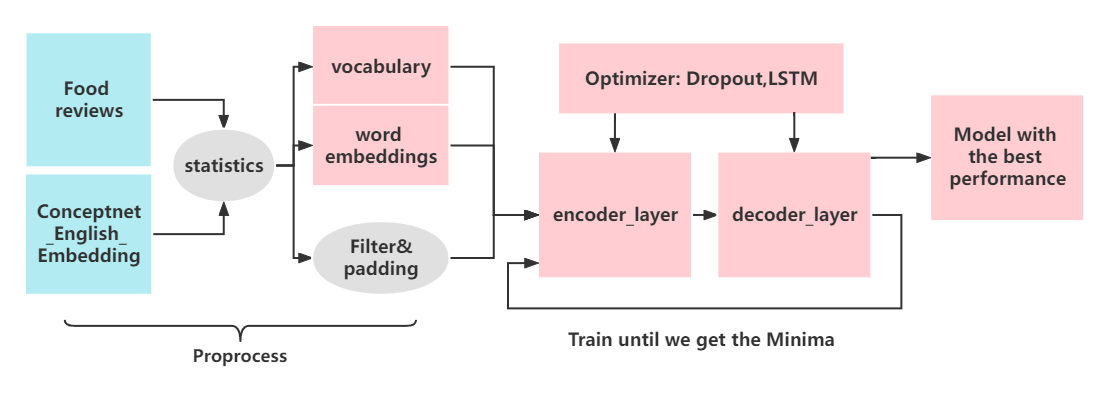
\includegraphics[width=0.5\textwidth]{imgs/System_Structure.png}
\caption{System structure}
\label{fig:System_Structure}
\end{figure}
\begin{flushleft} 
We implemented the following steps using PyTorch.
\end{flushleft}
\subsection{Data Preparation}
This dataset consists of more than 50,000 Amazon reviews of fine foods posted over a 10-year period from October 1999 to October 2012. It contains information about the product ID, user ID, profile name, helpfulness numerator, helpfulness denominator, review score, time, summary, and text. Here, “text” represents reviews that customers provided; for ease of understanding, we rename “text” to “reviews.” \\
\indent Before cleaning the data, we load the dataset using pandas. For this project, we focus only on the summary and review columns, so the other columns are being dropped, and null values are being removed. We then replace contractions with their full/longer forms using the list posted on~\cite{unknown}. We also convert every word of the summaries and reviews to lowercase and remove any unwanted characters, such as the dash, hyphen, and @. We import the Natural Language Toolkit (NLTK), which includes a list of 40 stop words, into our model. We only remove stop words from the reviews because they are not too important to the training process. By doing so, the size of the dataset is reduced, which speed up the training process. After cleaning the summaries and reviews, we use ConceptNet Numberbatch (CN) to map words to word embeddings. If certain words do not exist in CN, we assign the words to UNK tokens. Before sorting the reviews and summaries by length from shortest to longest, we add a GO token and an EOS token at the front and end of each sentence respectively. To obtain more meaningful data, if the UNK tokens appear more than once in the descriptions or more than 0 times in the summaries, the reviews are being removed. At this point, we are ready to build a model.

\subsection{Build a Model}
\indent We use a seq2seq model with an encoder and decoder architecture. We want to train the model in batches, so we define a function to create mini batches. Additionally, if sentences are shorter than the maximum length of a sentence within a mini batch, we pad zeros at the end of the sentence after the EOS token to ensure that the lengths are the same. Here, the batch size is 64. \\
\indent The encoder takes in vocab size, hidden size, and dropout rate. For each sentence in a batch, the encoder takes the entire input sequence word by word and then generates a sequence of outputs and hidden states using the Gated Recurrent Unit (GRU). The GRU is also known as a method to solve the vanishing gradient problem. It consists of an update get and a reset gate, which helps the model determine how much past information it should pass along or forget. At each time step, the hidden state takes information from the previous time steps’ outputs and inputs. Then, when we reach the last hidden state, it still contains vital information from before. The encoder will return a sequence of outputs for each sentence and the last hidden state. The last hidden state is also called the context vector. The decoder also takes in the vocab size, hidden size, and dropout rate. The hidden size and dropout rate for the encoder and decoder are the same, which are 100 and 0.2, respectively. The context vector from the encoder is the input for the decoder. The decoder produces the predicted summary word by word, and it will start after the GO token and stop when it reaches the EOS token. The decoder also returns all the hidden states for each sequence. \\
\indent For the final part, we build the seq2seq model. It takes in an encoder and decoder. It will produce a final prediction for each batch, and we use that prediction to compute the loss when starting training. 


\subsection{Train and Evaluate the Model}
Instead of training an entire dataset, which could be time consuming, we use a subset between 20,000 to 25,000. Therefore, we train median sequence lengths. We also randomly split the dataset into training and validation sets, and there is no overlap between the two datasets. The training set is for training purposes, and the validation set is for detecting whether the model underfit or overfit. To prevent gradient explosion, which occurs when large error gradients accumulate, resulting in extremely large updates to weights during training, we apply gradient clipping by norm. More specifically, it rescales gradients so that their norm will not exceed the threshold of 5 (we choose this value). For the optimizer, we use Adam to update weights more efficiently with a default learning rate of 0.001. Additionally, Cross Entropy (\ref{eqn1}) is used to evaluate the performance of the model. 
\begin{equation}
    \label{eqn1}
    L = - \dfrac{1}{N} \sum_{i = 1}^{N} y_i * log(p_i)
\end{equation}    
where $y_i$ is the target and $p_i$ is the prediction. We only compute the loss using the non zero elements on the target and prediction so we remove the padded zeros from them. 
For now, we set the number of epochs to 20, so the model will stop after running the entire training dataset 20 times.  \\ \\ 
\indent Moving forward, we will implement early stopping, which would stop the model if loss is not decreasing anymore and also prevent overfitting. Furthermore, we plan to create a profanity filter, apply an attention mechanism with LSTM to boost the accuracy of the model, and plot a graph to show the training and validation error.


\section{Evaluation Plan}
\subsection{Real datasets}
The dataset we use is Amazon Fine Food Reviews which contains more than 500000 records, spanning a period of more than 10 years. This dataset also provides summaries labeled by humans so that we can train our model to learn this ability to generalize. 
\subsection{Evaluation Measurement}
we will use both metric-based and human-subject evaluations to evaluate our model. Since we get the original summaries in the datasets, we can subjectively judge whether machine-generated generalization results outperform humans.  Besides, the performance of various text summarization methods is reported on shared DUC datasets using an automatic evaluation framework, ROUGE, which is DUC’s official evaluation metric for text summarization. We can also mix DUC with the original dataset and retrain our model to evaluate based on score.
\bibliographystyle{IEEEtran}
\bibliography{references.bib}



\end{document}
